%
% Copyright (C) 2004-2009 Jason Blevins <jrblevin@sdf.lonestar.org>
% http://jblevins.org/projects/cv-template/
%
% You may use use this document as a template to create your own CV
% and you may redistribute the source code freely. No attribution is
% required in any resulting documents. I do ask that you please leave
% this notice and the above URL in the source code if you choose to
% redistribute this file.

\documentclass[letterpaper, 9pt]{article}

\usepackage{hyperref}
\usepackage[dvipscol]{xcolor}

\definecolor{myteal}{HTML}{00B0F0}

\newcommand{\myorange}{myteal!70!black}
\newcommand{\darkorange}{\myorange !50!black}

\renewcommand{\bf}{\bfseries\color{\myorange}}
\renewcommand{\textbf}[1]{{\bfseries\color{\myorange}#1}}

% Function for highlighting text
\newcommand{\hl}[1]{{\color{darkgray}{\bfseries{}#1}}}

\usepackage{geometry}
\usepackage[minbibnames=4,maxbibnames=4,sorting=ydnt,date=comp,isbn=false,doi=false]{biblatex}
\addbibresource{papers.bib}

\AtEveryBibitem{%
	\clearfield{note}%
}

\DeclareSortingTemplate{ndymdt}{
	\sort[direction=descending]{
		\field{sortyear}
		\field{year}
		\literal{9999}
	}
	\sort[direction=descending]{
		\field[padside=left,padwidth=2,padchar=0]{month}
		\literal{99}
	}
	\sort[direction=descending]{
		\field[padside=left,padwidth=2,padchar=0]{day}
		\literal{99}
	}
	\sort{
		\field{presort}
	}
	\sort[final]{
		\field{sortkey}
	}
	\sort{
		\field{sortname}
		\field{author}
		\field{editor}
		\field{translator}
		\field{sorttitle}
		\field{title}
	}
	\sort{
		\field{sorttitle}
	}
	\sort[direction=descending]{
		\field[padside=left,padwidth=4,padchar=0]{volume}
		\literal{9999}
	}
}

\usepackage{graphicx}
\usepackage{enumitem}

%\usepackage[sfdefault]{cabin}
%\usepackage[T1]{fontenc}

%\usepackage[sfdefault]{overlock} %% Option 'sfdefault' only if the base font of the document is to be sans serif
\usepackage[default,oldstyle,scale=0.95]{opensans}
\usepackage[T1]{fontenc}

% Reduce spacing 
\usepackage{setspace}
\setstretch{0.95}

% Set your name here
\def\name{George G. Vega Yon, Ph.D.}

% Replace this with a link to your CV if you like, or set it empty
% (as in \def\footerlink{}) to remove the link in the footer:
\def\footerlink{https://ggvy.cl}

% The following metadata will show up in the PDF properties
\hypersetup{
  colorlinks = true,
  urlcolor = \myorange,
  pdfauthor = {\name},
  pdfkeywords = {economics, statistics, mathematics},
  pdftitle = {\name: Curriculum Vitae},
  pdfsubject = {Curriculum Vitae},
  pdfpagemode = UseNone
}

\geometry{
%  body={6.5in, 9in},
  left=1cm,
  top=1cm,
  right=4.5cm,
  bottom=1cm
}

% Not justified text
\raggedright

% % Customize page headers
\usepackage{fancyhdr}
%\pagestyle{myheadings}
%\markright{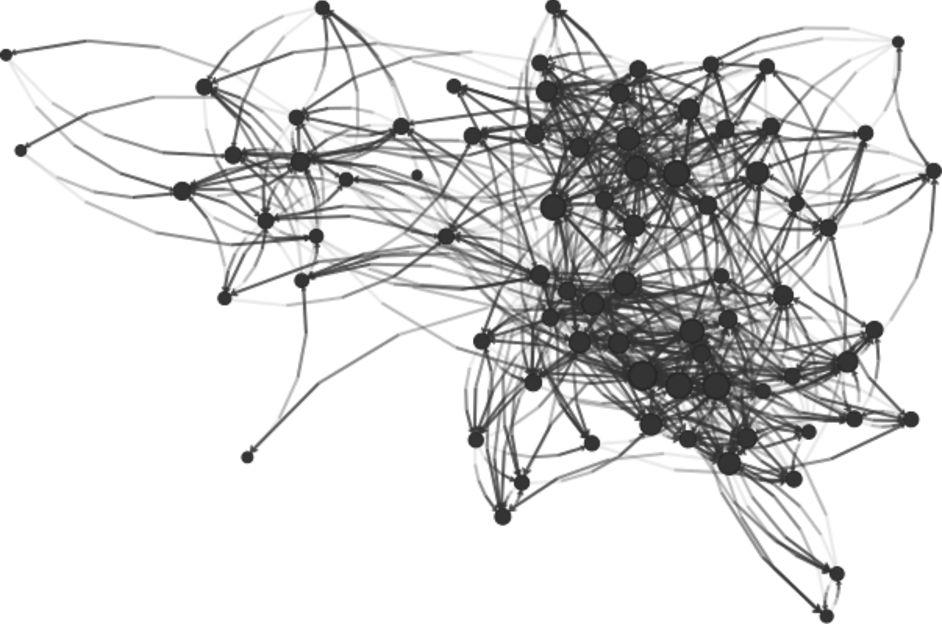
\includegraphics[width=1cm]{fig/ukfaculty.pdf} \name}
\pagestyle{fancy}
\fancyhead{}
\fancyfoot{}
\renewcommand{\headrulewidth}{0pt}
% \fancyhead[L]{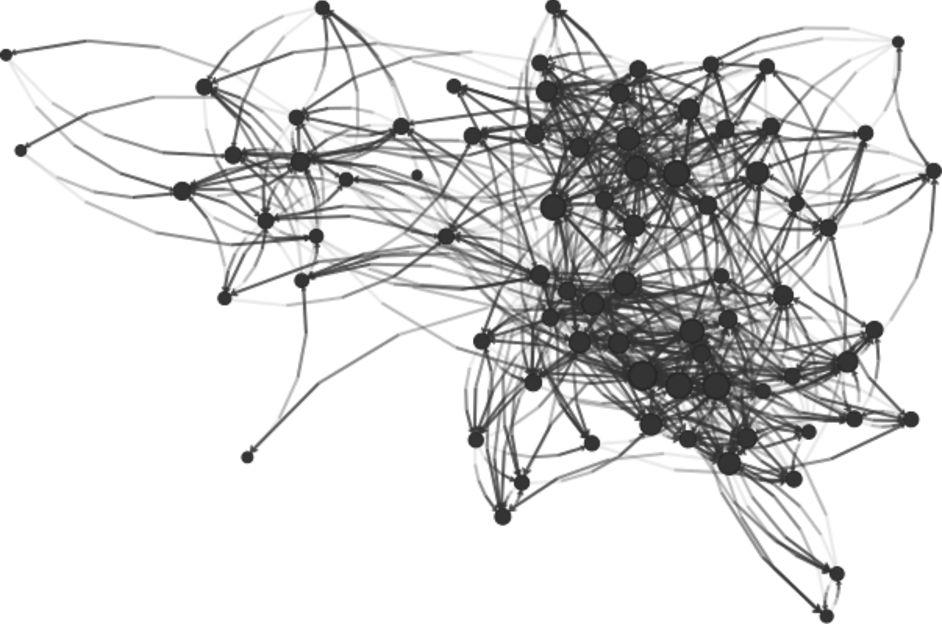
\includegraphics[width=1cm]{fig/ukfaculty.pdf}\\\vspace{-.75cm}\hspace{1.1cm}\emph{\name}}
% \fancyhead[R]{\small\thepage}
\thispagestyle{empty}

% Custom section fonts
%\usepackage{sectsty}
%\sectionfont{\sffamily\mdseries\Large}
%\subsectionfont{\sffamily\mdseries\itshape\large}

% Other possible font commands include:
% rmfamily
% \ttfamily for teletype,
% \sffamily for sans serif,
% \bfseries for bold,
% \scshape for small caps,
% \normalsize, \large, \Large, \LARGE sizes.

% Don't indent paragraphs.
\setlength\parindent{0em}

% Make lists without bullets
\renewenvironment{itemize}{
  \begin{list}{}{
    \setlength{\leftmargin}{0.3cm}
  }
}{
  \end{list}
}

% Para poder poner comandos genericos en tablas (en el inicio del argumento)
\usepackage{array}

\usepackage{tikz}
\usetikzlibrary{positioning}

\begin{document}
	
\begin{tikzpicture}[remember picture, overlay]
	\node[anchor=north east, inner sep=30pt] at (current page.north east) {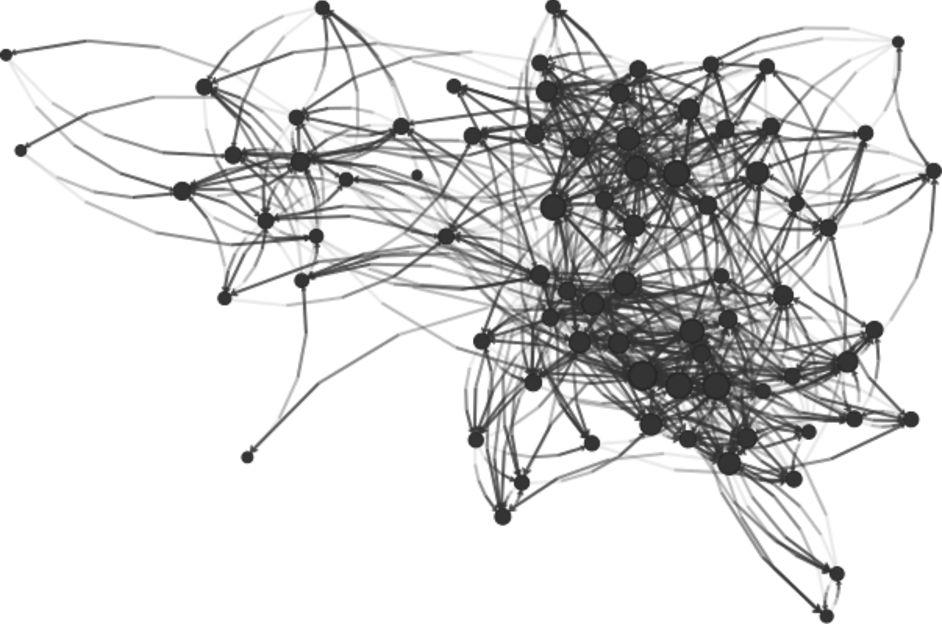
\includegraphics[width=0.35\textwidth]{fig/ukfaculty.pdf}};
\end{tikzpicture}

% embed a pdf page



\begin{tikzpicture}[remember picture, overlay]
	\node[anchor=north east, inner sep=80pt] (A) at (current page.north east) {};%
	\node[below=5pt of A, inner sep=20pt] (B) { %at (current page.east) {%
	% 
\includepdf[pages={1}]{fig/hexlogos.pdf} %
	\href[]{https://github.com/gvegayon}{
\includegraphics[width=0.25\textwidth]{fig/hexlogos.pdf}
	}};
	% Adding a node with text right below the previous node
	\node[below=20pt of B] {%
	\begin{minipage}{0.25\textwidth}
		\small
		\raggedleft \color{darkgray}
		\textbf{Technologies} R, C++, \LaTeX, SQL, Python, XML, regex, Stata, AWS, Gephi, Pajek, Mathematica, Git, Docker, Visual Studio Code, tensorflow, continuous integration, Slurm, Unix, Jira.
		
		\bigskip

		% \textbf{Skills} Statistical Analysis, Simulation, Data Visualization% 
		% 	}
	\end{minipage}
	};
\end{tikzpicture}

% \begin{tikzpicture}
% 	\node[anchor=east, inner sep=20pt] at (current page.east) {%
% 	
% \end{tikzpicture}
	% % Place name at left
	% \hfill 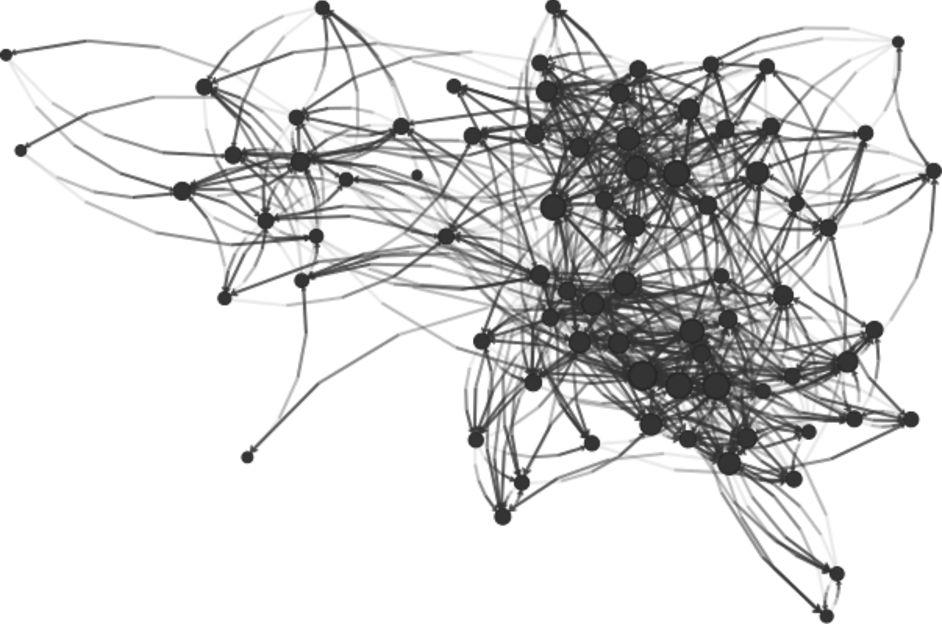
\includegraphics[width=.4\linewidth]{fig/ukfaculty.pdf}
	\vspace{-1.75cm}
	\part*{\color{darkgray}{\name} } 
	
	\vspace{-.4cm}
	\color{darkgray}{\textit{Data Science, Statistical Computing, \& Complex Systems Modeling}}
	\bigskip


	\begin{minipage}{.9\linewidth}
	\raggedright
	I'm an accomplished \textbf{data scientist} with over \textbf{10 years of experience} with multiple software packages and scientific publications. My software has been downloaded over \textbf{half a million times}, and my papers have over \textbf{200 citations}. My work has spanned data science, economics, network science, statistics, and phylogenetics. I seek new challenges, enjoy collaborating with others, and excel at mentoring.
	\end{minipage}

	\bigskip

% Alternatively, print name centered and bold:
%\centerline{\huge \bf \name}

%\vspace{0.25in}

\begin{minipage}{0.50\linewidth}
  \begin{tabular}{>{\bfseries}p{.2\linewidth}p{.79\linewidth}}
    Mobile & +1 (six two six) 381 8171 \\
    e-mail & \href{mailto:g.vegayon@gmail.com}{\tt g.vegayon@gmail.com} \\
    website & \href{https://ggvy.cl}{\tt ggvy.cl} \\
    Code & \href{https://github.com/gvegayon}{\tt github.com/gvegayon}\\
    Linkedin & \href{https://www.linkedin.com/in/georgevegayon/}{\tt www.linkedin.com/in/georgevegayon/} %\\
    %Talks & \href{https://ggv.cl/talk}{\tt ggv.cl/talk}
  \end{tabular}
\end{minipage}

\vspace{-.25cm}
\section*{\color{\darkorange}{Education}}
\vspace{-.25cm}

\begin{itemize}
\item 
{\bf Ph.D. in Biostatistics (Stat. Comp.)} University of Southern California (2020).

{\bf M.Sc. in Social Sciences (Economics)} California Institute of Technology (2016)

{\bf MA in Economics and Public Policy}, Universidad Adolfo Ib\'a\~nez (2011)

{\bf BS. in Business Administration}, Universidad Adolfo Ib\'a\~nez (2011)
\end{itemize}

\vspace{-.6cm}
\section*{\color{\darkorange}{Professional Experience}}
\vspace{-.3cm}

\begin{itemize}
\item \textbf{University of Utah, November 2021--Present} Department of Internal Medicine\\
\emph{Research Assistant Professor in Epidemiology}\\
\emph{Adjunct Assistant Professor in Population Health Sciences}. 
\begin{itemize}
	\item[-] \hl{Research} areas: Mechanistic ML, Network Science, Computational Epidemiology, Phylogenetics, Statistical Computing.
	\item[-] \hl{Managed} a group of research assistants (staff and graduate students), leading to published papers, software, and conference talks.
	\item[-] \hl{Taught} and designed the first course on HPC using R and C++ (graduate level).
	\item[-] \hl{Founder} of the "Network Science and Social Network Analysis at the U" (NetSNAU) Group.
	\item[-] \hl{Contributed} to research grants (CDC and VA,) helping to secure over \hl{1 MM USD in funding}.
	\item[-] Core faculty member of the \hl{"Utah Center for Data Science"}.
\end{itemize}
\item \textbf{University of Southern California, 2018--2021} Department of Preventive Medicine\\\emph{Research Programmer II}.
\begin{itemize}
	\item[-] Provide technical support on \hl{software development} (R packages), HPC, R, and C++, including training sessions for staff and students.
	\item[-] \hl{Write} scientific papers on network science, statistics, and phylogenetics and present them at conferences.
	\item[-] \hl{Designed} and taught the course "Intro to Health Data Science" (graduate level).
	\item[-] Contributed to \hl{research grants} (NIH and DoD,) helping to secure over \hl{10 MM USD in funding}.
\end{itemize}
\item \textbf{University of Southern California, 2015--2018} Department of Preventive Medicine\\\emph{Programmer Analyst II}. 
\begin{itemize}
	% \item[-] Wrote R package for Social Network Analysis.
	\item[-] \hl{Organized} local conferences on Network Science.
	\item[-] \hl{Founder} of the "R Bookcamp for Statistical Computing." 
	\item[-] \hl{Wrote} scientific papers and software on network science and presented them at conferences.
	\item[-] Designed and \hl{led workshops} on R and Social Network Analysis.
\end{itemize}
\item \textbf{Chilean Pension Supervisor, August 2011-- August 2014} Research Division\\
\emph{Research Analyst}
\begin{itemize}
	\item[-] Wrote papers and automatized \hl{statistical reports} about the Chilean unemployment insurance system.
	\item[-] \hl{Managed administrative data} (\textit{e.g.}, social security) and created representative samples for researchers.
	\item[-] Designed and implemented a \hl{pipeline for simulation and forcasting} of the unemployment insurance government funds. Reports were distributed to the Chilean Congress.
\end{itemize}
% \item \textbf{Universidad Adolfo Ib\'a\~nez, January 2011--June 2012.} School of Government \emph{Adjunct Professor}.
% Taught Introductory courses of Economics, Microeconomics and Statistical computing with Stata.
\end{itemize}

\newgeometry{left=1.3cm, right = 1.3cm, top = 1.3cm, bottom = 1.3cm}

\section*{\color{\darkorange}{Software {\small (selected)}}}
\vspace{-.25cm}

\begin{enumerate}[label={[}\arabic*{]},labelindent=5\parindent,labelsep=8pt]
\item {\bfseries George G.} {\bfseries Vega Yon}. \textit{{aphylo: Statistical Inference of Annotated Phylogenetic Trees}} (2022). R package version 0.2-1 {\small URL}: \url{https://cran.r-project.org/package=aphylo}. 
\includegraphics[width=2.5cm]{fig/cran-downloads-aphylo.pdf}
\item {\bfseries George G.} {\bfseries Vega Yon}. \textit{rgexf: Build, Import and Export GEXF Graph Files} (2020). R package version 0.16.0. {\small URL}: \url{https://CRAN.R-project.org/package=rgexf}. 
\includegraphics[width=2.5cm]{fig/cran-downloads-rgexf.pdf} 
\item {\bfseries George G.} {\bfseries Vega Yon}, Thomas Valente. \textit{{{netdiffuseR: Analysis of Diffusion and Contagion Processes on Networks}}} (2020). R package version 1.22.0. {\small URL}: \url{https://github.com/USCCANA/netdiffuseR}. 
\includegraphics[width=2.5cm]{fig/cran-downloads-netdiffuser.pdf} 
\item {\bfseries George G.} {\bfseries Vega Yon}, Kayla de la Haye. \textit{ergmito: Exponential Random Graph Models for Small Networks} (2020). R package version 0.3-0. {\small URL}: \url{https://cran.r-project.org/package=ergmito}. 
\includegraphics[width=2.5cm]{fig/cran-downloads-ergmito.pdf} 
\item {\bfseries George G.} {\bfseries Vega Yon}. \textit{slurmR: A Lightweight Wrapper for 'Slurm'} (2020). R package version 0.4-1. {\small URL}: \url{https://CRAN.R-project.org/package=slurmR}. 
\includegraphics[width=2.5cm]{fig/cran-downloads-slurmr.pdf} 
\item {\bfseries George G.} {\bfseries Vega Yon}. \textit{fmcmc: A friendly MCMC framework} (2020). R package version 0.3-0. {\small URL}: \url{https://CRAN.R-project.org/package=fmcmc}. 
\includegraphics[width=2.5cm]{fig/cran-downloads-fmcmc.pdf} 
%\item {\bfseries George G.} {\bfseries Vega Yon}. \textit{barry: your to-go motif accountant} (2020). C++ library version 0.0-1. {\small URL}: \url{https://github.com/USCbiostats/barry}.  
\end{enumerate}

\nocite{yon2019exponential,VegaYon2019c,VegaYon2019a,vegayon2020aphylo,vegayonPowerMulticollinearitySmall2023,vegayonDiscreteExponentialFamilyModels2022} %VegaYon2019b
\section*{\color{\darkorange}{Academic Publications {\small (selected)}}}
\vspace{-.25cm}

\printbibliography[title=\vskip-20pt,omitnumbers=true]


\section*{\color{\darkorange}{Honors and Professional Achievements}}
\vspace{-.25cm}

\begin{itemize}
% \item \textbf{Book reviewer}: ``Microeconometrics and Matlab: An Introduction'', by Adams, Clarke and Quinn, Oxford University Press, 2015. ``Mastering Gephi Network Visualization'', by Ken Cherven, Packt Publishing, 2015. ``Network Graph Analysis and Visualization with Gephi'', by Ken Cherven, Packt Publishing, 2013.
\item \textbf{Awards} Best paper, 72 ICA conference, 2022; Travel Grant, Society of Young Network Scientist, 2019; Fellowship, California Institute of Technology, 2014; Scholarship, Adolfo Ib\'a\~nes University, 2006.
%\item \textbf{Book reviewer} ``Microeconometrics and MATLAB'', by Abi Adams, Damian Clarke \& Simon Quinn, Oxford University Press, (forthcoming 2015).
\item \textbf{Manuscript reviewer} JASA, BMC Infectious Diseases, The Official Journal of The Society for Computational Economics, The R Journal, Social Networks, Journal of Mathematical Sociology, JOSS, Bioinformatics, Computer Methods and Programs in Biomedicine Update, SUNBELT Conference (2016), IC2S2 (2019--2021).
\item \textbf{Misc} Founder of the \href{https://www.meetup.com/useRchile/}{R Users Group in Chile (2013)}, co-organizer of the \href{https://socalr.org}{East LA R User Group (LAERUG)}.
%\item \textbf{Honorable Mention} (Posters Sesion. Work: \emph{Introducing Parallel: Stata Module for Parallel Computing}) given by the Chilean Economics Society during its 2012 annual meetting.
%\item \textbf{Honour Scholarship} given by Adolfo Ib\'a\~nez University for completing undergrad and graduate studies (2006-2010).
%\item \textbf{Software workshop, 2010.} \emph{Co-founder} of the workshop thaught by Economics and PP Masters's Students at Adolfo Ib\'a\~nez University in order to introduce grad students into scholar research software (\LaTeX, \emph{R}, Stata, etc.).
\end{itemize}

% Footer
\begin{center}
 \begin{footnotesize}
   last update: \today \\
   \href{\footerlink}{\texttt{\footerlink}}
 \end{footnotesize}
\end{center}

\end{document}

